\documentclass[11pt]{article}

\usepackage{preprint}
\usepackage{amsmath, amsthm, amssymb, amsfonts}
\usepackage{resizegather}
\usepackage[numbers,square]{natbib}
\usepackage[utf8]{inputenc}
\usepackage[T1]{fontenc}
\usepackage{xcolor}
\usepackage[colorlinks = true,
    linkcolor = purple,
    urlcolor  = blue,
    citecolor = cyan,
    anchorcolor = black]{hyperref}
\usepackage{booktabs}
\usepackage{multirow}
\usepackage{nicefrac}
\usepackage{microtype}
\usepackage{lineno}
\usepackage{float}
\usepackage[shortlabels]{enumitem}
\usepackage{float}
\usepackage{subfloat}
\usepackage{caption}
\usepackage{subcaption}
\usepackage{amssymb}
\usepackage{bbold}
\usepackage{stmaryrd}
\usepackage{graphicx}
\usepackage{hyperref}
\usepackage{titlesec}
\usepackage{authblk}
\usepackage{graphics}
\usepackage[font=small,labelfont=bf]{caption}
\captionsetup[subfigure]{justification=centering}

\setlength{\belowcaptionskip}{-10pt}
\newcommand{\specialcell}[2][c]{%
  \begin{tabular}[#1]{@{}c@{}}#2\end{tabular}}


\bibliographystyle{unsrtnat}
\setlist[enumerate,1]{leftmargin=2em}
\titlespacing\section{0pt}{0.1ex plus 0.2ex minus 0.1ex}{0.1ex plus 0.2ex minus 0.1ex}
\titlespacing\subsection{0pt}{0.1ex plus 0.2ex minus 0.1ex}{0.1ex plus 0.2ex minus 0.1ex}

\renewcommand*{\Authfont}{\bfseries}

\newcommand{\R}{\mathbb{R}}
\newcommand{\N}{\mathbb{N}}
\DeclareMathOperator*{\argmin}{arg\,min}
\DeclareMathOperator*{\argmax}{arg\,max}
\DeclareMathOperator*{\minimize}{minimize}
\DeclareMathOperator*{\Argmin}{\text{Argmin}}

\title{Generative modeling project : Neural Optimal Transport}
\author[1]{Paul Barbier}
\author[1]{Bastien Le Chenadec}
\affil[1]{École des Ponts ParisTech, Master MVA}

\begin{document}

\maketitle

\begin{contribstatement}
\end{contribstatement}

\section{Introduction}

Optimal Transport (OT) is a mathematical framework that aims to find the most efficient way to transport a distribution of mass to another. This framework has been used extensively in the context of generative models, for instance as a loss function in the training of Generative Adversarial Networks (GANs) or by learning a mapping between two distributions. In this project, we aim to study the paper "Neural Optimal Transport" (Korotin, 2023) \cite{korotin-2022} which introduces an algorithm to train a neural network to learn the optimal transport between two distributions.

\section{Background on Optimal Transport}

Let $\mu$ and $\nu$ be two probability distributions on $\mathcal{X}$ and $\mathcal{Y}$ respectively (typically $\mathcal{X}, \mathcal{Y}=\R^n,\R^m$). To give a meaning to "efficiently" transporting mass, we need to define a cost function $c:\mathcal{X}\times\mathcal{Y}\to\R$ that quantifies the cost of transporting a unit of mass in $\mathcal{X}$ to one in $\mathcal{Y}$. The (Monge) optimal transport problem consists in finding a \textbf{transport map} $T^*:\mathcal{X}\to \mathcal{Y}$ such that :
\begin{equation}
    T^* \in \Argmin_{T\#\mu=\nu} \int_{\mathcal{X}} c(x,T(x))d\mu(x)
\end{equation}
where $T\#\mu$ is the pushforward distribution of $\mu$ by $T$, defined by $(T\#\mu)(A)=\mu(T^{-1}(A))$ for any measurable set $A\subset\mathcal{Y}$. This formulation calls for a deterministic mapping from $\mathcal{X}$ to $\mathcal{Y}$, which is not always desirable or feasible under general assumptions. Kantorovich introduced  a more general OT problem that aims at finding a \textbf{transport plan} $\pi^*\in \Pi(\mu,\nu)$ in the set of joint distributions on $\mathcal{X}\times\mathcal{Y}$ with marginals $\mu$ and $\nu$ such that :
\begin{equation}
    \pi^* \in \Argmin_{\pi\in\Pi(\mu,\nu)} \int_{\mathcal{X}\times\mathcal{Y}} c(x,y)d\pi(x,y)
\end{equation}
In general the solution to the Kantorovich problem is stochastic, but in some cases it may be deterministic in which case it is also a solution to the Monge problem. Following this idea of stochasticity in the solution, weak OT was introduced as a relaxation of the Kantorovich problem, where the cost function is of the form $C: \mathcal{X}\times \mathcal{P}(\mathcal{Y})\to\R$. In this case the weak OT problem writes :
\begin{equation}
    \pi^* \in \Argmin_{\pi\in\Pi(\mu,\nu)} \int_{\mathcal{X}} C(x,\pi(\cdot|x))d\pi(x)
\end{equation}
where $\pi(\cdot|x)$ is the conditional distribution of $\pi$ given $x$ and $d\pi(x)$ is the marginal distribution of $\pi$ on $\mathcal{X}$.

Building on this framework, (Korotin, 2023) \cite{korotin-2022} introduce \textbf{stochastic maps} $T:\mathcal{X}\times \mathcal{Z}\to \mathcal{Y}$ where $\mathcal{Z}$ is a latent space corresponding to the randomness in the transport. They show that the weak optimal transport problem can be reformulated and solved by a SGAD algorithm. This approach is particularly interesting in the context of generative modeling, as it allows to learn a stochastic mapping between two distributions.

\section{Experiments}

For this project, we conducted experiments using the code provided by the author. You can find our scripts at \href{https://github.com/bastienlc/NOT}{https://github.com/bastienlc/NOT}. We've done a first experiment with generated synthetic data and a second one with a more realistic use-case using a large dataset.

\subsection{Synthetic data}

\subsection{Real dataset}

Authors made experiments using faces from animes and real persons and the results were funny so we decided to make a similar one with a different dataset. More precisely, we took the CelebA dataset~\cite{celeba_dataset} which comprises 200k images of celebrity faces with attribute annotations. For the second dataset, we chose CartoonSet100K, a dataset introduced in~\cite{cartoonset_dataset}. It's a large-scale dataset containing 100k of 2D generated cartoon avatar images. 

\begin{figure}[h!]
    \centering
    
\includegraphics[scale=.2]{figures/cartoonset-excerpt.png}
    \caption{Images samples from CartoonSet100K}
\end{figure}

For this large-scale experiment we used a cloud instance with a NVidia A100 GPU with 40GB of memory. We increased the batch size per dataset from 64 to 128 and we used $128\times128$ images in place of $64\times64$ to get generated images with a nicer resolution. Increasing the batch size lead to better memory utilisation and quicker convergence as we'll see in the next paragraphs.

On the figure below, you can see how the loss function evolves throughout the training. Unusually, the loss function here is fluctuating around the constant value 0 and that's expected: explain why it's expected TODO.

\begin{figure}[h!]
    \centering
    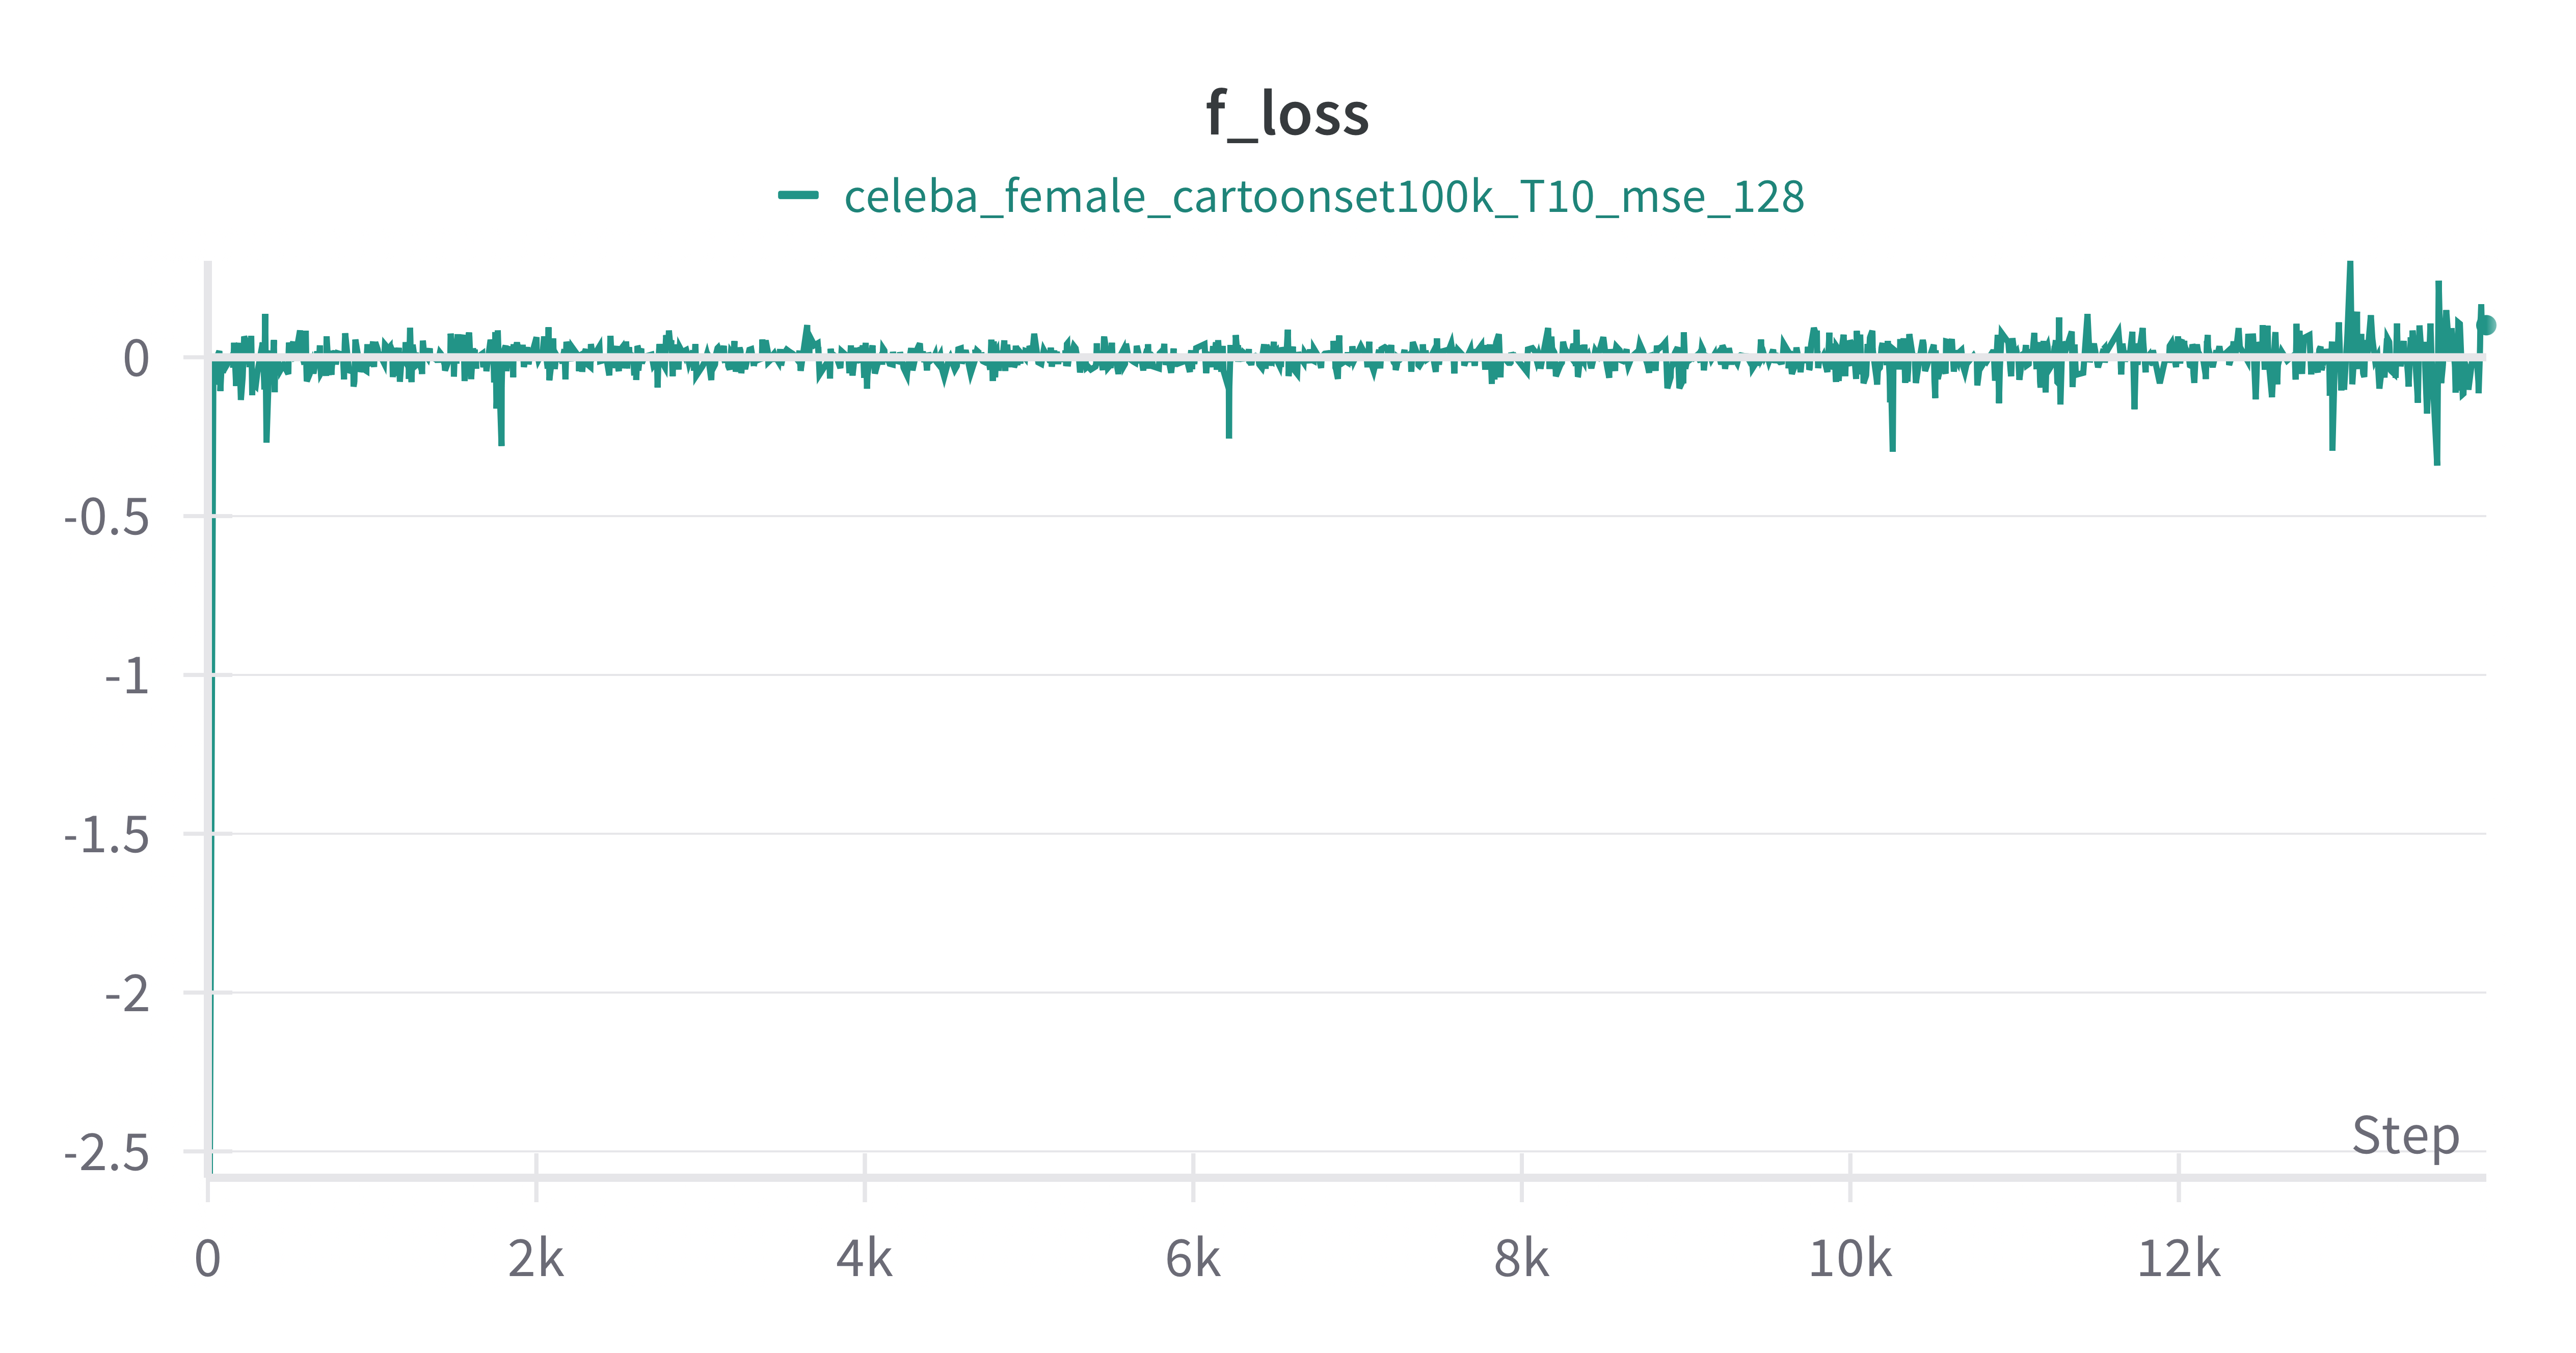
\includegraphics[scale=.05]{figures/loss_real_dataset.png}
    \caption{Loss function}
\end{figure}

\begin{figure}[htp!]
    \centering
    \begin{subfigure}{\textwidth}
        \centering
        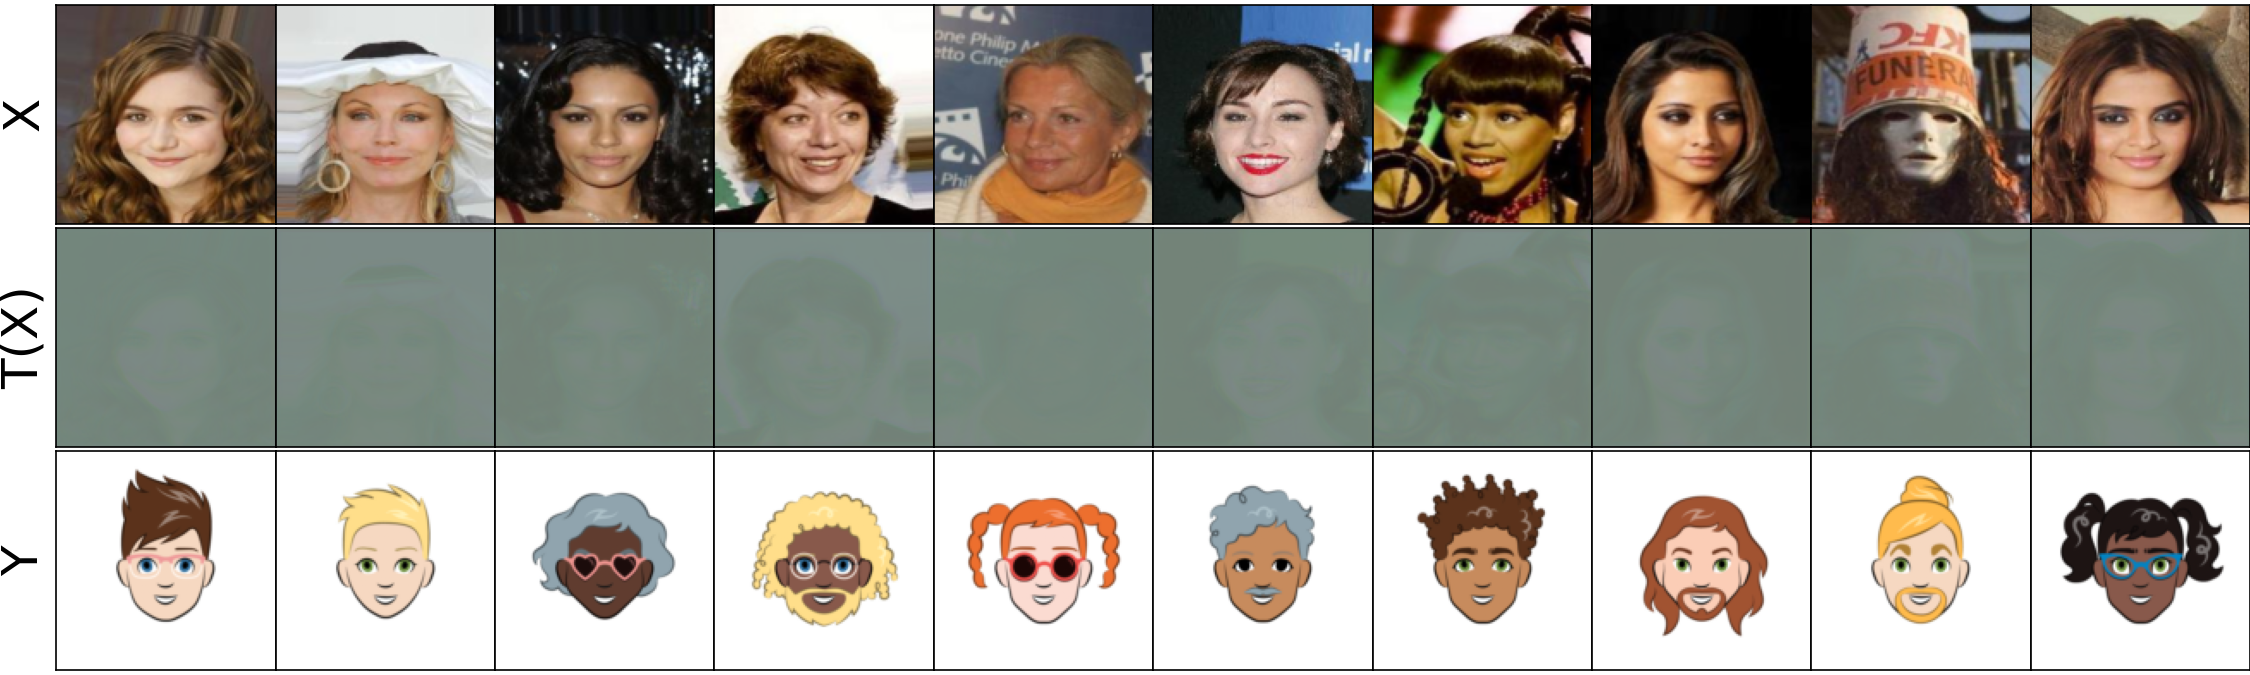
\includegraphics[scale=.15]{figures/media_images_Fixed Images_0_a56284c48d003ecfb6cd.png}
        \caption{Iteration 1}
        \label{fig:test_images_real_iter_1}
    \end{subfigure}%
    
    \bigskip

    \begin{subfigure}{\textwidth}
        \centering
        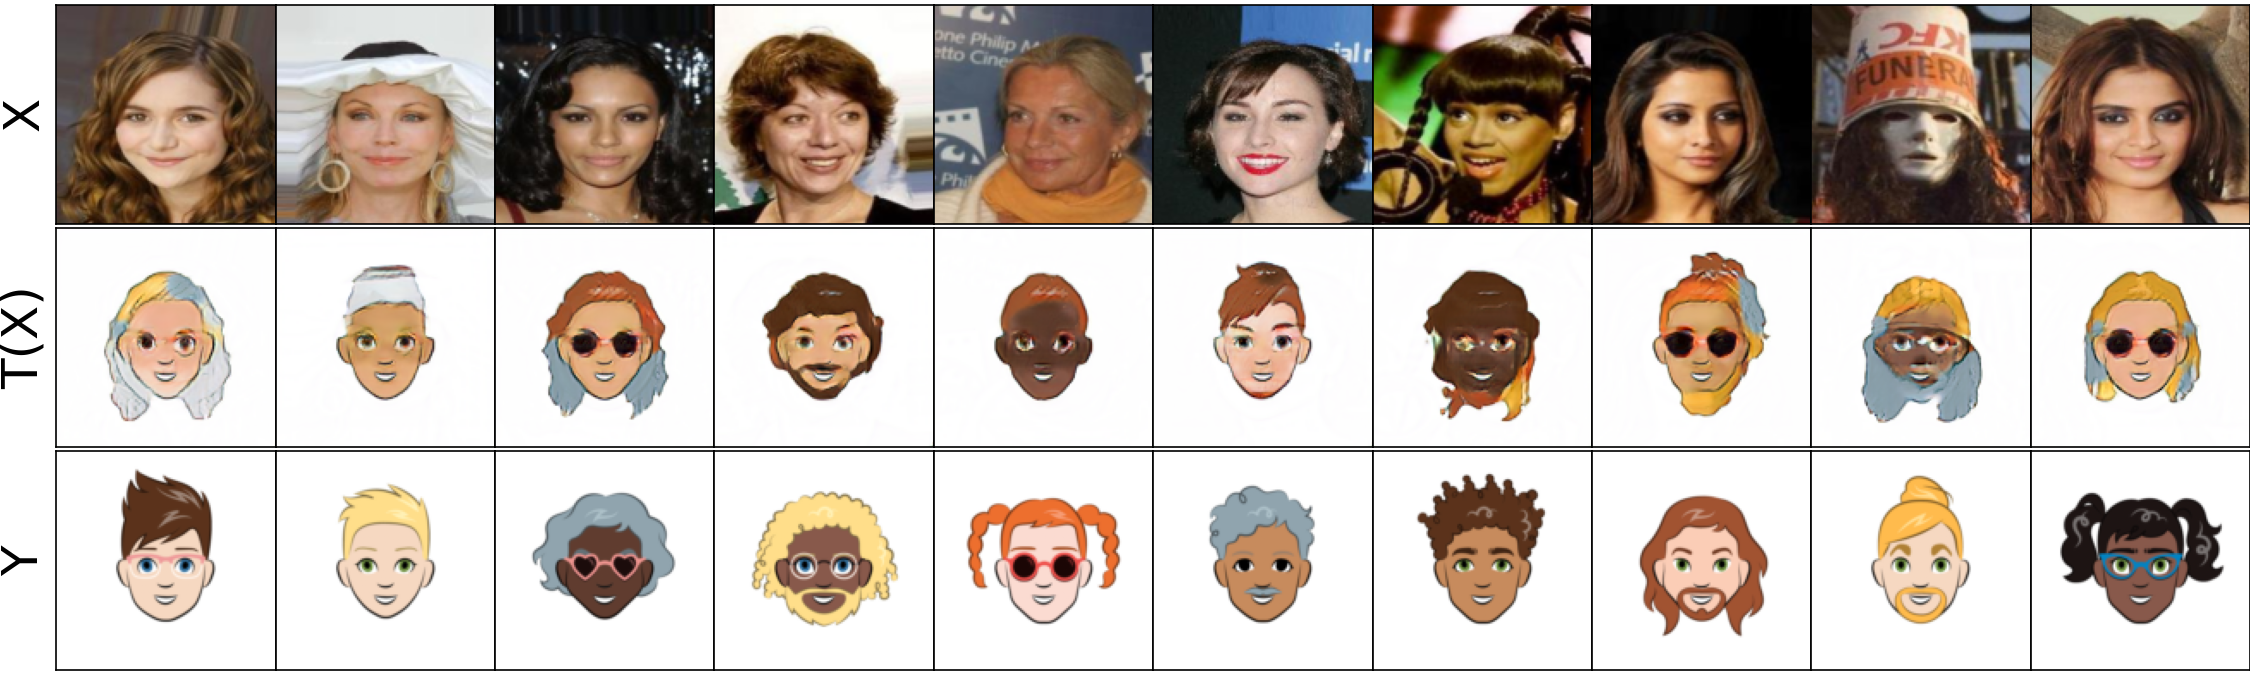
\includegraphics[scale=.15]{figures/media_images_Fixed Images_5000_0043c7527d827202e7ad.png}
        \caption{Iteration 5000}
        \label{fig:test_images_real_iter_med}
    \end{subfigure}%

    \bigskip

    \begin{subfigure}{\textwidth}
        \centering
        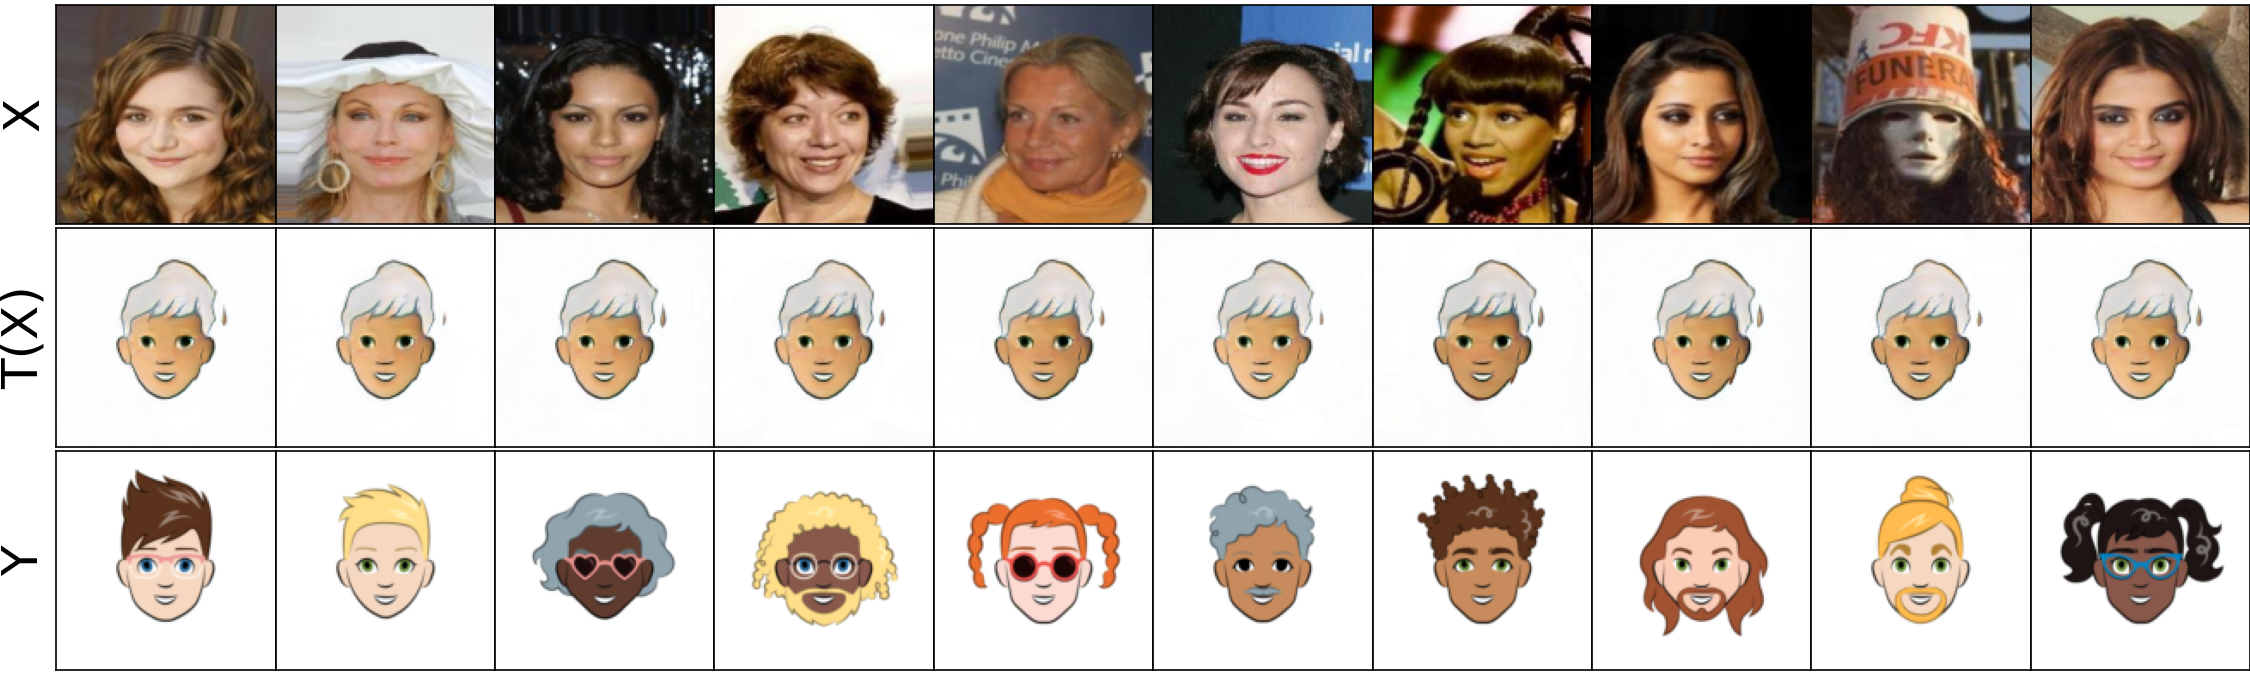
\includegraphics[scale=.15]{figures/media_images_Fixed Images_13800_653d5de40c4ba6a777ca.png}
        \caption{Iteration 13800}
        \label{fig:test_images_real_iter_last}
    \end{subfigure}%
    \caption{Test images}
    \label{fig:test_samples_large_scale}
\end{figure}

Those experiments are quite long in time (about a day for \~15k iterations with the parameters given above) so we restrict ourselves to only train the strong formulation model and the results for a fixed sample of the test set are given in~\ref{fig:test_samples_large_scale}.

\subsubsection{Observations}

Figure~\ref{fig:test_images_real_iter_1} lets us see the model initialisation.

Furthermore, we witnessed realistic mappings of the real faces onto the cartoon avatar distribution around iteration 5000, see~\ref{fig:test_images_real_iter_med}. This is far less than what the authors observed in their experiments, this number was closer to 40k iterations for convergence. However, our images have an empty background so it might be easier in comparison with anime face images which contain a complex surrounding as they are extracted from animes. One can see that the color of the skin and the hair map well. However, the model struggles when there are glasses on the target image. It translates glasses into dark black holes. It's very surprising to see new avatars thanks to those mappings.

At this point, we thought we were far from the end and we decided to continue the training for a night. Unfortunately, few thousands iterations later mode collapses appeared with the same avatar being mapped for a given batch. Surprisingly, the constant predicted face is changing with training without changing the mode collapse.

\section{Conclusion}

Random sentence for the conclusion in the meantime.

\newpage
\bibliography{bibliography}

\newpage
\appendix

\begin{center}
    {\Large \bfseries \scshape Appendix} \\
\end{center}

\section{Figures}

\end{document}
